\documentclass[]{article}

%opening
\title{Malicious context and workaround analysis of decentralized VPN:\\the case of Mysterium Network}
\author{Jacopo Federici}


\usepackage{imakeidx}
\usepackage{setspace}
\usepackage{url}
\usepackage{graphicx}
\makeindex

\begin{document}
	\setstretch{1.0}
	\maketitle	
	\clearpage
	
	\tableofcontents{}

	\subsection{Note}
	parlare di:
	\begin{itemize}
		\item docker (cosa è, comandi base per fare cosa)
		\item robe di networking per dev mode del progetto:
		\begin{itemize}
			\item https://www.digitalocean.com/community/tutorials/a-deep-dive-into-iptables-and-netfilter-architecture
			\item http://www.naturalborncoder.com/virtualization/2014/10/17/understanding-tun-tap-interfaces/
			\item http://linux-training.be/networking/ch14.html
		\end{itemize}
	\end{itemize}
	\section{parte introduttiva}
		
	\subsection{Abstract}
	\subsection{Work structure}
	\subsection{Outline}
	\subsection{Goal}
	
	
	\section{State of art}

	\subsection{Introduction}
	The need for privacy is becoming more critical day after day.
	The massive digitalization of many aspects of our life implicitly exposes us and our data and eve the simplest operations which use an internet connection are becoming unsafe.
    In the last years, we have seen security solutions integrated into popular applications, such as browsers or mobile apps, following the increase of security attacks. For instance, in 2017, the popular Chrome browser announced it would mark as non-secure any website using the HTTP protocol instead of HTTPS. This move was to encourage the website to use SSL/TLS certificates and make secure the communication between client and server. It's interesting to discover the Netscape Navigator browser has made the first HTTPS version around 1990, but the official RFC publication has been released only in May 2000 \cite{HTTPS}. ((Why has this solution been largely used only fifteen years later?))
    Similar scenario for the VPN: abbreviation for "virtual private network" it's a technical solution to extend a private network across a public network. It is created by establishing a virtual point-to-point connection through the use of dedicated circuits or with tunneling protocols over existing networks. Many of the VPN implementations encrypt the traffic between the two points. A first VPN specification proposal can be dated around 2000 \cite{VPNRFC}, but only in the last years, the use of VPN is becoming massive. The data encryption feature solves privacy problems the VPN was not intentionally designed for, such as crossing a censored network rather than use services available only in certain countries.
    Currently, many commercial solutions allow users to have a private connection between their computer and the company servers across the world. In this way, the user can have access to the internet resources from the position around the globe he prefers, skipping firewalls, proxies, and other tracking and censure methods applied by some companies or countries.
    There are many security concerns about those commercial solutions, such as the ability of the VPN provider to keep logs, inspect the traffic, or sell statistic data obtained by the users.
    Some open-source projects were, lately, born to solve these problems. Their goal is to revolution the idea of VPN and its uses, building a rich network of peers where two nodes can connect through a VPN. The project provides a platform that includes all the components needed to have an efficient, fast, and easy-to-use system: from the discovery to the payment.
    
    In this research document, we analyzed the most developed project, Mysterium Network, as a case of study. As we write, Mysterium offers a working network composed of hundreds of nodes around the world, making it the best project to investigate malicious contexts and design vulnerabilities on, owns by the decentralized architecture, more than the Mysterium project itself.
	We even discover how secondary aspects are pivotal to guide attacks to the system.
    The second step focuses on the solutions that can be implemented to patch those critical aspects and provides a comparison between different solutions with an eye on the practical perspective.
	
	\subsection{The world now}
	We still are in the middle of a huge transformation. Since the invention of the pc and the born of the internet. More and more services are becoming digital; more and more people are using those services; more and more bad guys are trying to pull down those services.

	But there are differences from some decades ago.
	First, everything is now much faster. The internet infrastructure can grant us to move significant amounts of data within a few seconds, and access to online services is used and necessary. 

	Furthermore, our personal computer can perform operations only some years ago were impossible to execute on mainstream servers. This speed is finding the limits of many security solutions, such as ciphers that based and still do, their strength on the amount of time needed to reverse the encryption.
	Second, the architecture is changing back to a cloud-based infrastructure. Many workflows see, again, a thin client sending the execution step on a cloud server that elaborates the output to send back to the client. This architecture changes the attack surface addressing the cloud servers as the principal attack destinations.
	Third, some technologies are mature enough to provide an excellent alternative to traditional models — for instance, the cryptocurrency model against the bank model. Here, the changes regard the paradigma, and the reasons behind these new approaches are much more than technological.

	The security noun is changing the meaning inside the people's minds, from "how thick is my bank caveau" to "how long my bank requires my new online account password".

	Million of users worldwide resort to security solutions to accomplish online operations of any sort. Unfortunately, the existing technologies often show their design vulnerabilities.

	\begin{verbatim}
	https://www.geeksforgeeks.org/need-of-information-security/
	https://www.hackerfactor.com/blog/index.php?/archives/868-Deanonymizing-Tor-Circuits.html
	\end{verbatim}
	
	\subsection{the need for trust and privacy}=
	\begin{verbatim}
		https://www.howtogeek.com/133680/htg-explains-what-is-a-vpn/
		https://www.forbes.com/sites/tjmccue/2019/06/20/why-use-a-vpn/#3f08d7105859
		https://www.investopedia.com/terms/b/blockchain.asp
		https://www.howtogeek.com/350322/what-is-ethereum-and-what-are-smart-contracts/
		
		https://en.wikipedia.org/wiki/Proof_of_work
		https://en.wikipedia.org/wiki/Proof_of_stake
	\end{verbatim}
	
	Anonymization: in every network systems, the anonymization is a tough challenge. Even more, if privacy is a crucial point. In some countries, the VPN is massively used to protect data from surveillance at any level, from a public unsecured wifi connection to the country ISPs. There are countries, the People's Republic of China, for instance, where censorship is present and where identity obfuscation is necessary. In these cases, the use of a VPN is remediation as long as a safe company provides it. With the adjective "safe", we mean a company that does not make detectable your traffic into his network, or even worst sniffs and crafts your traffic for malicious actions. 

	The decentralized VPN completely changes the paradigma, the infrastructure design.
	A similarity can be made with the traditional bank model: as we know, the bank is a centralized entity trusted by definition. What if the bank suddenly becomes untrusted? Cryptocurrencies spread the trusts all of us put in the bank on ourself, cryptocurrency participants, using a blockchain as a technical solution. 
	A similar design is used with decentralized VPN: there is no central entity to control the system, but a significant number of peers, the network, we can choose to connect to based on different indexes.
	\subsection{We are our trust}


	\section{My work, steps}
	\subsection{Decentralized VPNs}
	\subsubsection{Introduction}
		
	\begin{verbatim}
		concetti introduttivi
		- blockchain in linea di massima\\
		- ethereum in linea di massima e descrizione degli smart contracts\\
		- proof of work, proof of stake\\
		- reputazione in una net (Eigentrust)\\
		- - cercare applicazione pratica di Eigentrust\\
		- descrizione di BFT\\
	\end{verbatim}

	A decentralized VPN is a network of nodes where the users can connect through a VPN to nodes without a centralized entity. The decentralization system, in this context, includes several steps to make the final connection happening, rather than a simple VPN connection between two peers.
	First of all, the user creates an identity into the system, linked to the payment wallet, using a client application. Then, it connects to the network providing its availability such as consumer or provider. The consumer user chooses the provider node he prefers based on the node's region, its quality, or its cost and asks for a new connection to that node. In this step, the blockchain, based on Ethereum, allows creating a smart contract between the two participants with a predetermined amount of money. Using commercial VPN applications, such as OpenVPN or Wireguard, the connection between consumer and provider, even called client and server, is established. When the connection correctly ends, the network closes the smart contract, and a result of the transaction is registered in the blockchain. 
	We have outlined the main steps from which we can deduce a decentralized VPN is more a platform solution rather than a simple VPN application. Indeed, other projects suggested the VPN is one of the functionalities a decentralized system like this can have. (EXPLAIN BETTER THE IDEA)  
		          
	\subsubsection{The business idea}
	As a business project, which aims to earn money, it has a specific business plan shared with similar projects: provide a system network where users can join as a service provider, selling their internet bandwidth, or as a service consumer, buying other's internet bandwidth. Each couple of entities, a consumer and a provider, agree on a transaction paid using cryptocurrency in the face of the used service. This transaction is ruled by an Ethereum smart contract signed by both of the sides. To close the transaction, a fee to the system must be paid. This fee is not the Ethereum smart contract fee, generally called gas, but the Mysterium source of earnings. For this reason Mysterium and other projects realized an internal market with a private coin (for Mysterium is called MYST) used to buy and sell internet bandwidth between the nodes inside the network. It's possible to convert MYST to ETH like a regular cryptocurrency.
	Altought the consumer can be the provider and vice-versa, the two entities a clearly different. This makes the type of market a two-sided market where bid and ask respectively grow on the other side growth. 

	
	(It's the typical market for digital goods and usually only one actor tends to dominate more than half of the market.)
		
	The main open-source projects are Mysterium Network, Privatix, Substratum and Sentinel. We explored all of them and we discovered the four different approaches they implement to reach the goal: building a distributed network based on blockchain with a discovering system, a crypto coin payment method, a mobile and desktop application.
	We can safely say the most advanced project is Mysterium Network, in terms of development and design. Furthermore it's 100\% open source, that for this kind of project is an important quality which conditions the users adoption and market diffusion.
	Therefore, we decide to use Mysterium Network as a test case to implement our proof of concepts.
	
	\subsubsection{Mysterium Network}
	
	Mysterium Network is an open-source project. Its main goal is to build a decentralized infrastructure made up of layered VPN protocols, blockchain, and smart contracts.

	As a general workflow description, Mysterium starts by collecting all the agents' service proposals and presents them to the clients. Then registers the client's intention to pay for the agent's service chosen by the user and creates the VPN connection between the two points.
	The outcome of each transaction is saved in the blockchain. In this manner, it's possible to rebuild the transaction history for any specific user, be it a consumer or a producer.
	
	The architecture is composed of four core components:
	Ethereum Blockchain allows running decentralized code with smart contracts, enabling reliable and payment handling.
	Identity service and database of registered identities ensures the proper identity acknowledgment between client and service provider.
	Discovery service and database of available services provide means to announce VPN services availability and pick the most suitable VPN service.
	Payment service and database of balances allow secure promise-based micropayments for services.

	\begin{figure}
		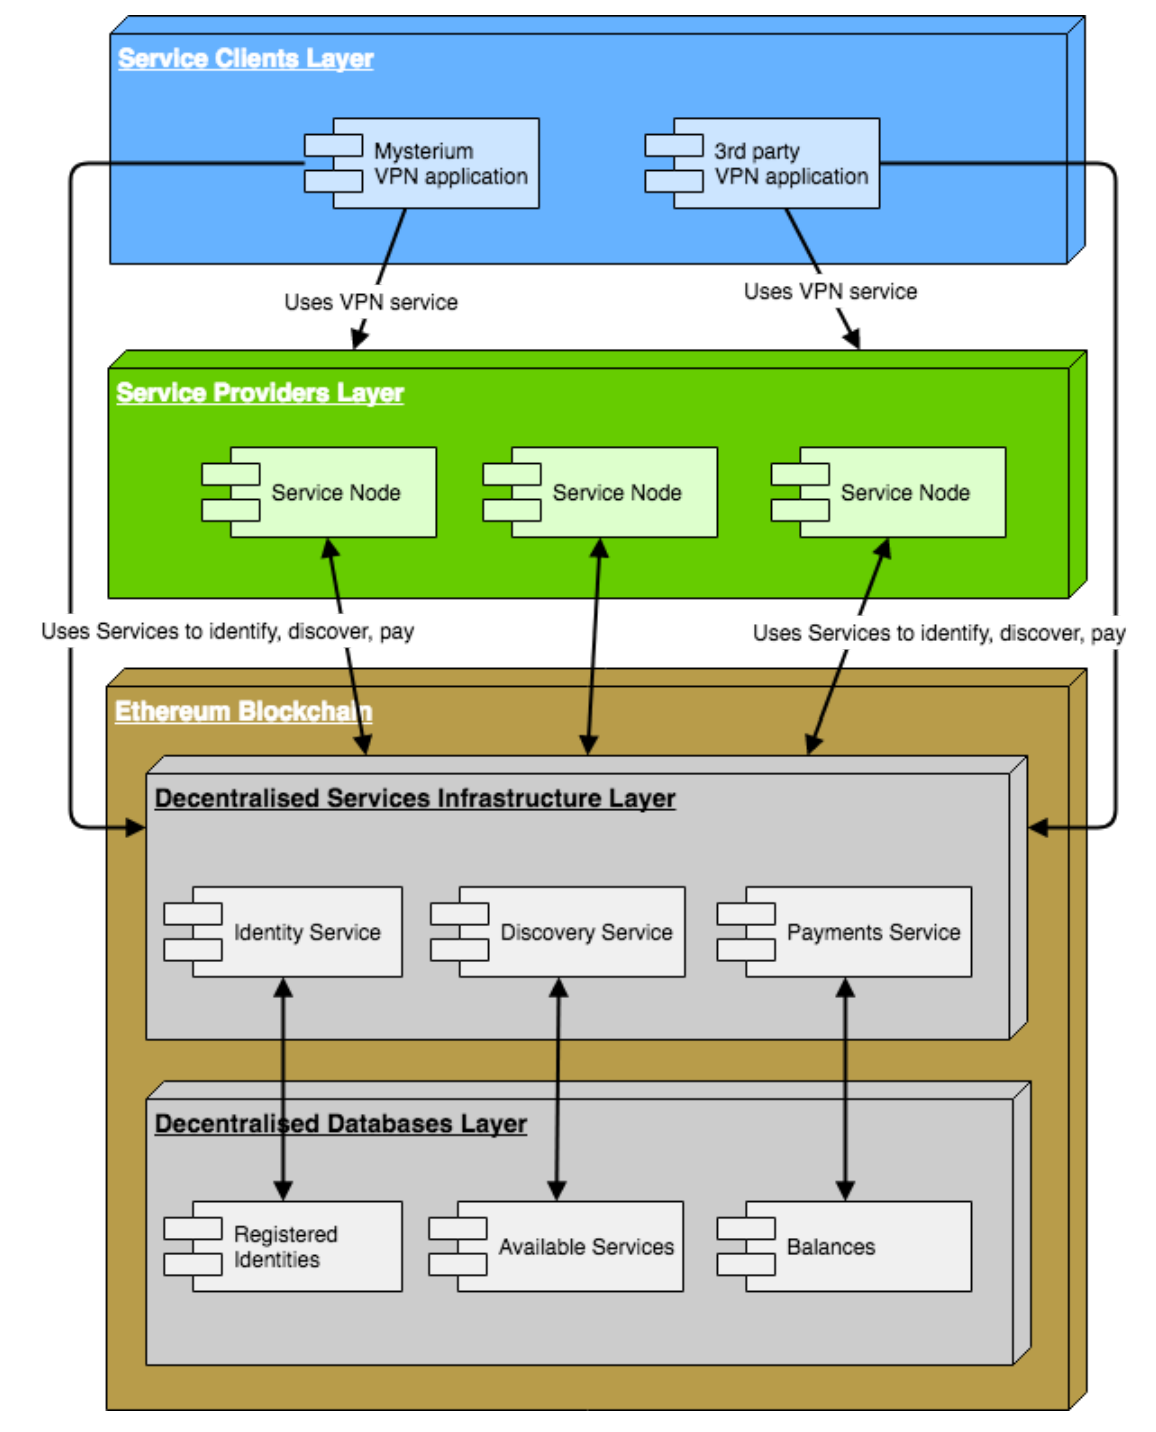
\includegraphics[width=\linewidth]{"images/mysterium_architecture.png"}
		\caption{A boat.}
		\label{fig:boat1}
	\end{figure}

	The Identity Service: the identity represents that every node needs can create one identity or more. Each identity consists of a public and a private key, and the last 20 bytes of the hash function, applied on the public key, is the unique public ids. To publish it so that other network members can reach it, Mysterium uses the smart contract mechanism. In such a way, identities are registered in the blockchain after the miners elaborate it. The private and public keys are used to validate the signature for the communication between the nodes. 

	The mining process appends the public key and the unique id to the Ethereum blockchain and takes fees the nodes must pay to the network. 
	This amount of money has the purpose of giving value to the identity. In such a way, it is unattractive to abandon it, expensive, but not impossible. 
	We will discuss those aspects later, but we can surely say this is the first barrier to make prohibitive in mass identity creation. 
	Furthermore, the user benefits using the same identity because it is possible to rebuild its transaction history and its balance from the Ethereum blockchain, making him more predictable and thus trustworthy for service providers. 

	\begin{figure}
		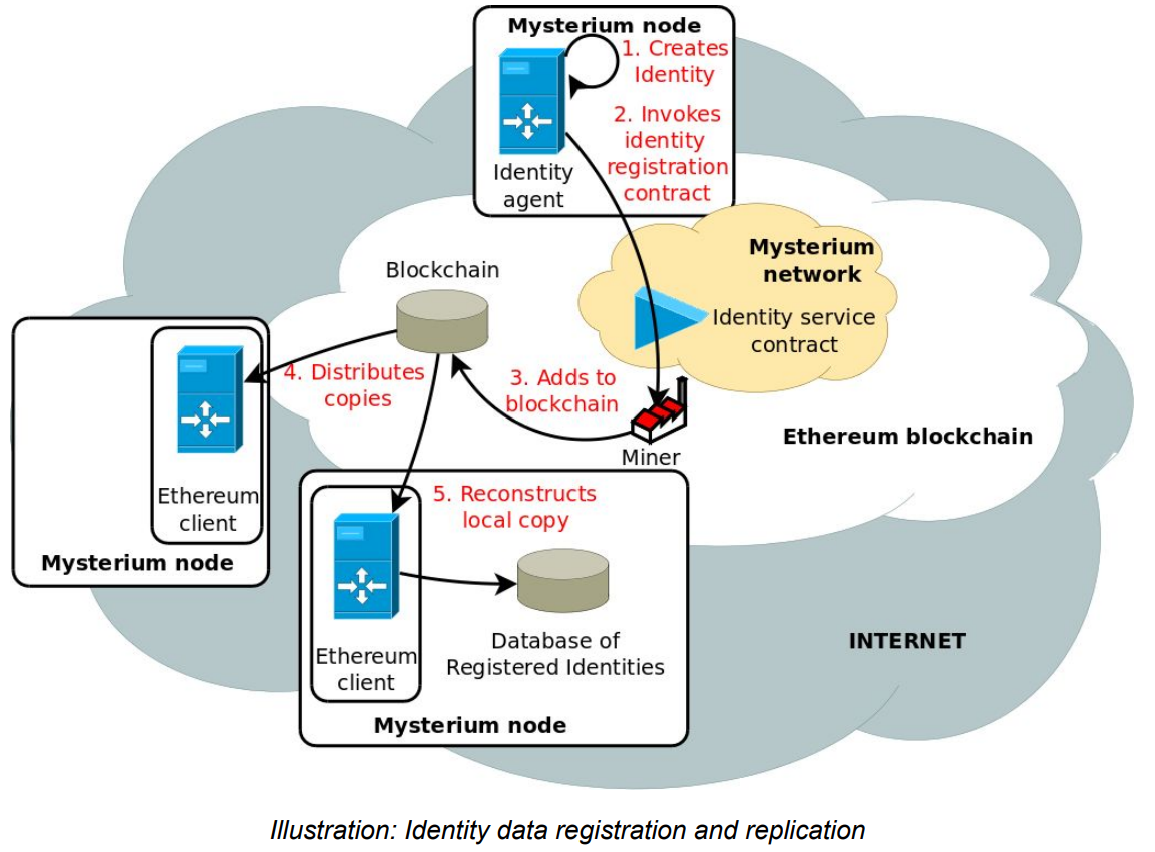
\includegraphics[width=\linewidth]{"images/mysterium_identity_creation.png"}
		\caption{A boat.}
		\label{fig:boat1}
	\end{figure}

	The Service Discovery: it provides the list of service proposals available in the network. The service needs to announce its availability posting the proposal characterized by service parameters depending on proposed services. The parameters can be the VPN application it supports, the server's connection IP address and port, the provider's server location, or the bandwidth per session. Then, the miners append it to the blockchain, making it publicly available for everyone.

	
	\begin{figure}
		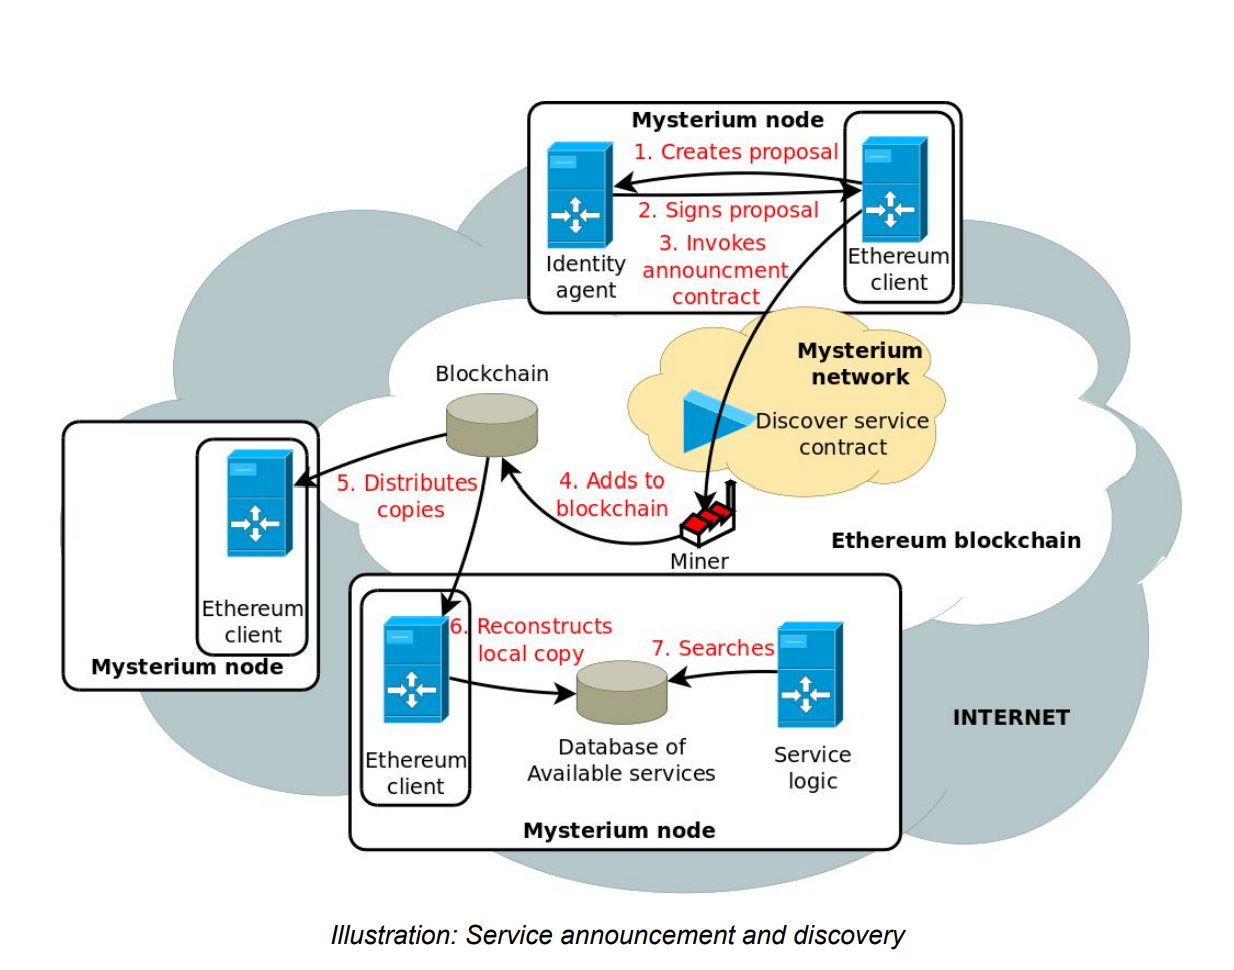
\includegraphics[width=\linewidth]{"images/mysterium_service_announcement.png"}
		\caption{A boat.}
		\label{fig:boat1}
	\end{figure}

	
	Payments Handling: Ethereum blockchain holds all the mechanisms for the payment steps, and everyone needs an account managed by the smart contracts to operate in the Mysterium Network. To advance a request, the consumer has to have enough cryptocurrency in his wallet. If so, he can ask for a connection to a producer who has previously published a service proposal. Mysterium calls this step a promise creation because the client effectively promises he will pay when the service ends.  Positively clearing a promise is the interest of everybody, producer, and consumer, since a canceled promise marks the consumer's history hitting his reputation for future connections.


	Architecture: the core application is called "node". It's written in GoLang, a new program language made by Google that is having a high adoption in the last years. The node creates a local webserver to connect to the network, manages the cryptocurrency wallet, and initiates the VPN connection as a client or manages the incoming connection as a server. Mysterium does not implement its version of VPN but leans on famous VPN applications, which are OpenVPN and Wireguard. 
	It can be run in two modes, as a client or as a server, and is managed via command-line interface or via RESTful API exposed in the localhost, called TequilaAPI. TequilaAPI is used by the client application to manage the connection and for diagnostic operations. Mysterium developed a desktop client written using Electron, a technology that is a web application locally executed by NodeJs, a server backend.
	The node is also available as Docker image ready-to-use and published on the Docker Hub. 
	On the mobile side, Mysterium is present with its multiplatform app that works only as a client.


	Project setup: 
	Note: from now on, we refer to the consumer even as the client and the producer even as the server, both of them related to the VPN connection.
    Note: the platform used for our research is Linux based, and even if some details are different, they share the same logic, and so the VPN used implementation is OpenVPN, but similar deductions can be made on Wireguard or other VPN applications.


    When the promise is created, the communication between the two nodes starts. The client node begins the connection to the server node with the chosen VPN application. 

	OPENVPN WORKING EXPLANATION: 
	
	\begin{verbatim}
		https://subscription.packtpub.com/book/networking_and_servers/9781783553136/1/ch01lvl1sec12/openvpn-internals
	\end{verbatim}

	The VPN server application creates a virtual interface where to encrypt and decrypt the traffic.

	\begin{figure}
		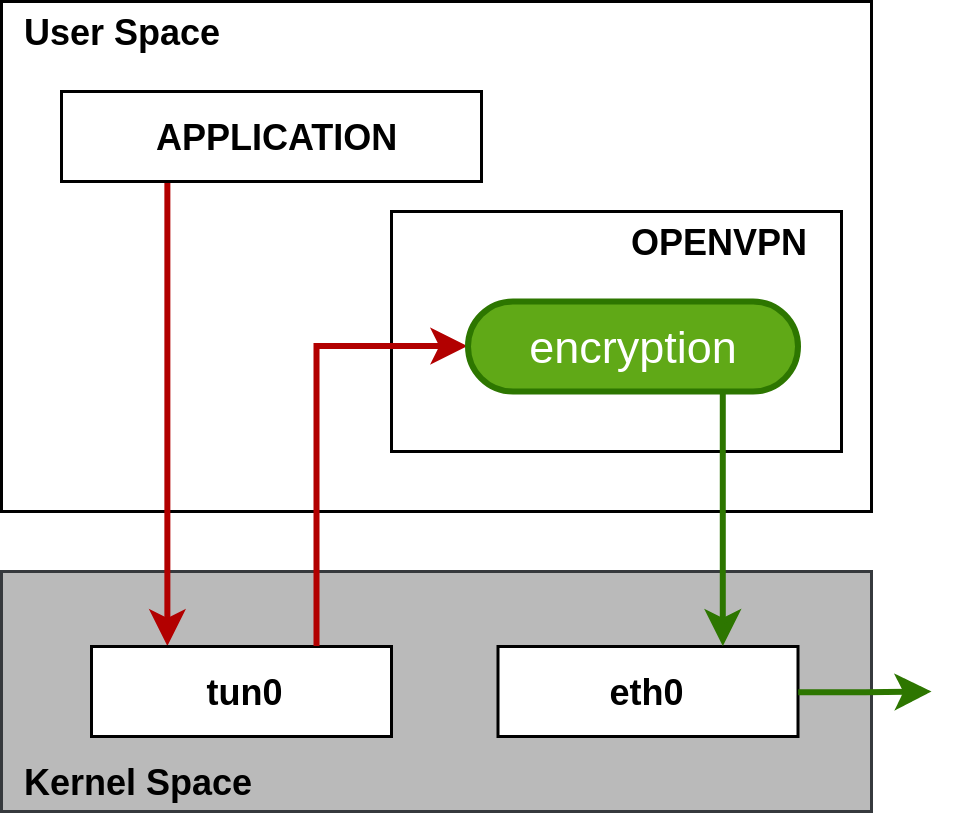
\includegraphics[width=\linewidth]{"images/openvpn_tun_interface.jpg"}
		\caption{A boat.}
		\label{fig:boat1}
	\end{figure}

	The server works as a proxy: forwards all the data that comes from the VPN tunnel to the internet and vice-versa.
	The client, on the other side of the tunnel, performs the same operations, but inverted. 

	\begin{figure}
		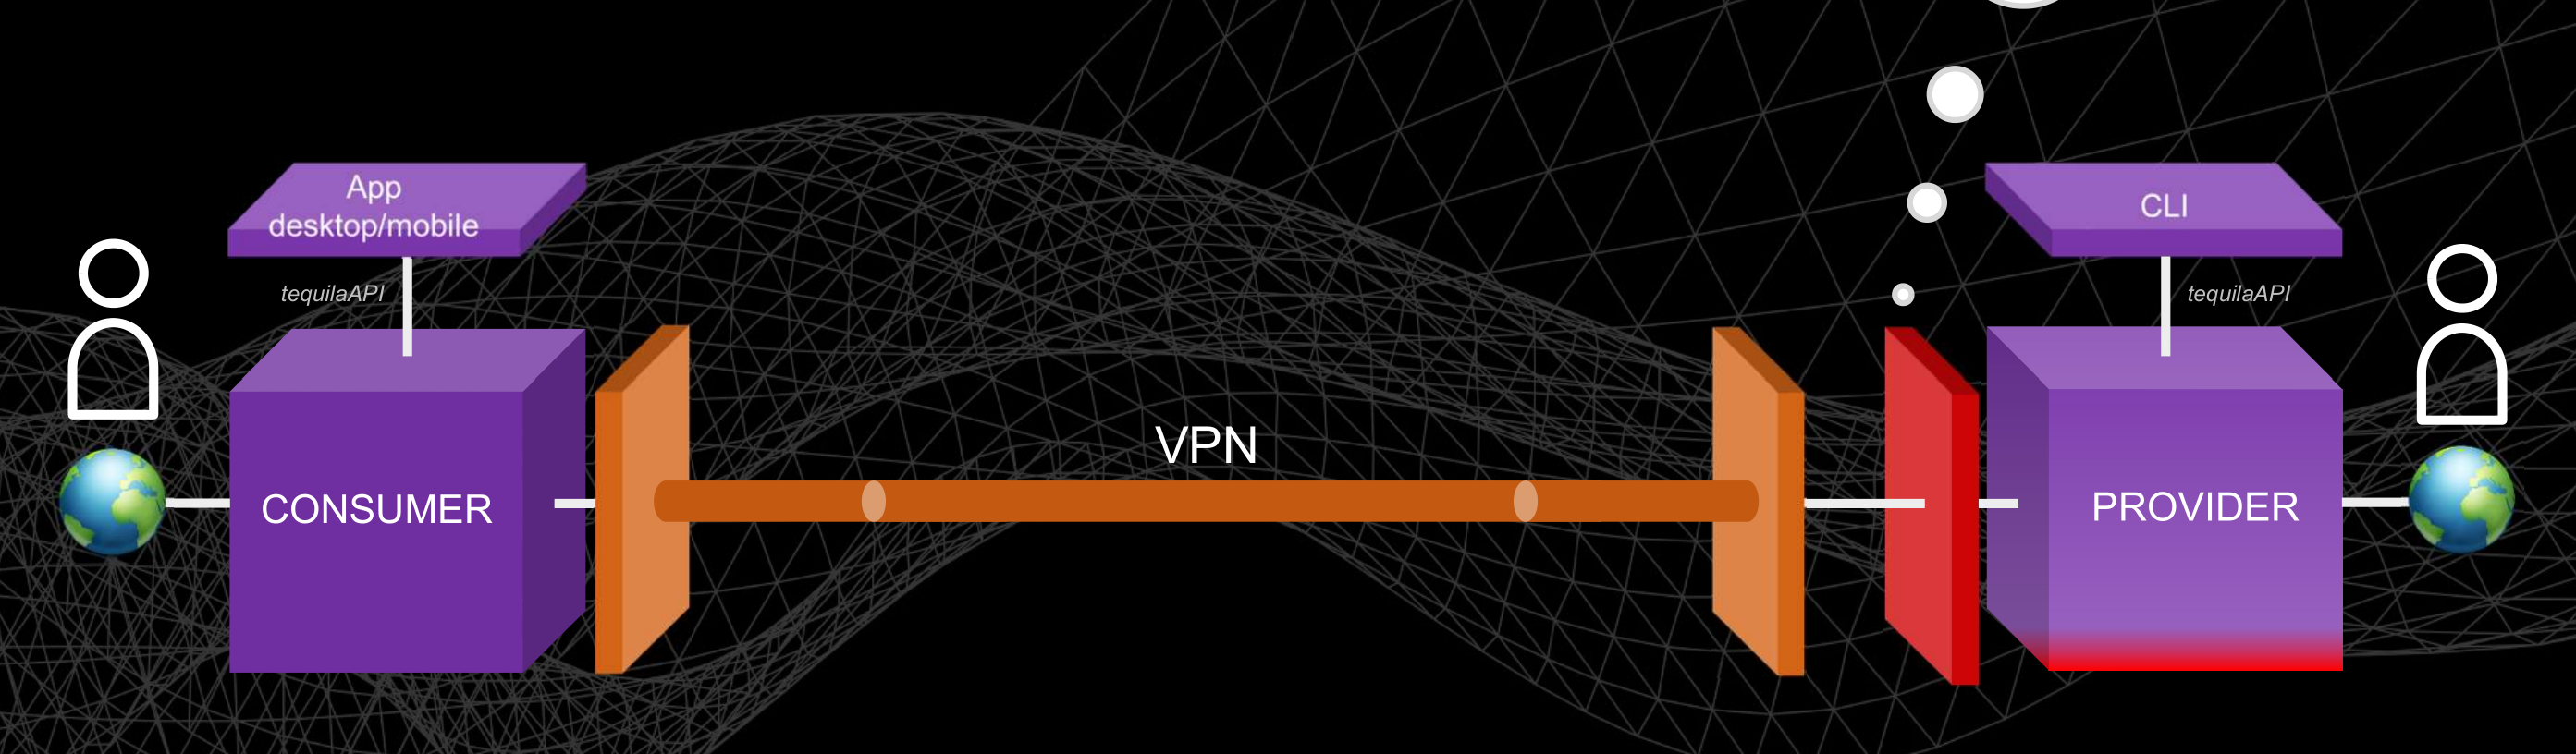
\includegraphics[width=\linewidth]{"images/client_server_vpn_connection.png"}
		\caption{A boat.}
		\label{fig:boat1}
	\end{figure}

	\subsection{Basic sniffing to catch content (Wireshark, tcpdump)}
	\subsection{Craftberry, a demo tool}
			useful tips
			\begin{verbatim}
				http://unixwiz.net/techtips/gnu-c-attributes.html
				https://gcc.gnu.org/onlinedocs/gcc-4.0.2/gcc/Type-Attributes.html
				https://groups.google.com/forum/#!msg/pcapplusplus-support/e7rN93LfTSg/MFnVEKCNCAAJ
				https://byt3bl33d3r.github.io/using-nfqueue-with-python-the-right-way.html
			\end{verbatim}
			
			\subsubsection{liv 2: arp, vlan tagging}
			\subsubsection{liv 3: ip, icmp}
			\subsubsection{liv 4: tcp/udp}
			\subsubsection{side attacks}
				- auditin/collezione dei dati sniffati, inviati ad un server esterno per collezionamento, statistiche, vendita a terzi.
				- trojan all'interno di craftberry, per botnet. (approfondire aspetto che se il sw di attacco diventa popolare, può essere lui stesso veicolo di malware, quindi attacco l' attaccante)
			
			\begin{itemize}
				\item copia x volte dei pacchetti (TCP/UDP)
				\item gonfiamento dei pacchetti nei campi che poi verranno corretti dai check (TCP/UDP)
				\item modifica del payload se in chiaro (TCP/UDP)
				\item azione positiva sul payload (UDP), ad esempio cifratura chacha20
			\end{itemize}
		 	\subsubsection{liv 5+: http/imap/dns/ntp/etc}
				analisi e modifica dei contenuti a livello del singolo protocollo (ad esempio sostituzione di tutte le immagini con una immagine di default)
			
	\subsection{Design solutions for malicious context}
		\subsubsection{comparing}
		invia la richiesta a due nodi e le confronta (essenziale possibilità di connessione a due nodi in contemporanea: due o più container docker mappati su porte diverse con uno script che invia la richiesta a più container e confronta le risposte)
		\subsubsection{comparing hashes}
		come precedente ma con la gestione degli hash invece che di tutto il dato
	\section{Design integration with reputation systems}
	
	\subsection{something here}
	
		
\section{Conclusions}
	\subsection{Tests}
	\subsection{Future development}
	\subsection{Considerations}

	\pagebreak

	\textbf{problemi individuati}
	\begin{enumerate}
		\item valutazione della reputazione dell'agent da parte del client
		\item valutazione della reputazione dell'agent da parte della Net
	\end{enumerate}
	
	\textbf{soluzioni proposta}
	\textbf{Proposte per la valutazione della reputazione dell'agent da parte del client}
	
	Le seguenti proposte sono metodi di verifica del corretto comportamento ed hanno come scopo finale la valutazione della reputazione degli agent
	\begin{itemize}
		\item Dati civetta: modifiche al client che con scadenze richiede una o più risorse dal valore noto e verifica che siano integre. Le scadenze possono essere regolari/random/all’inizio frequenti/dipendenti dalla reputazione dell’agent. È necessario avere delle risorse distribuite e disponibili: potrebbero essere i nodi stessi della rete (altri agent).
		\item Dati duplicati: modifiche al client che implementa la possibilità di connessione con più agent. Dopo la richiesta il client compara i dati ottenuti dalle due fonti
		\begin{itemize}
			\item Hash *: (soluzione aggiuntiva) I nodi sono generalmente in posizioni migliori dei client in termini di velocità. L’idea è quella di far generare un hash dei dati che il client richiede ad un altro nodo fuori dal servizio primario, così da comparare gli hash e non tutto il dato.
			Inoltre, se la richiesta la faccio a molti più nodi posso intrinsicamente verificare quali modificano i dati nel network.
		\end{itemize}
		\item Applicazione di modelli di reputazione (Eigentrust): attualmente non studiato
	\end{itemize}

	\bibliographystyle{plain}
	\begin{thebibliography}{1}
		\bibitem{HTTPS}
			https://tools.ietf.org/html/rfc2818
		\bibitem{VPNRFC}
			https://tools.ietf.org/html/rfc2764
		\bibitem{wikibook}
			manually managing references, 
			\url{https://en.wikibooks.org/wiki/LaTeX/Manually_Managing_References}
			2016
	\end{thebibliography}
		
	\pagebreak
	
	%%	{\Large Valutazione di un nuovo utente della rete}
	\paragraph{Contesto}
	Rete VPN decentralizzata attiva e con connessione multi-hop tra una generica coppia Agent-Client.
	
	\paragraph{Problema 1: identificare gli Agent in posizione endnode che inviano contenuto non originale}
	In una rete VPN decentralizzata gli Agent endnode hanno il compito di recuperare una risorsa web e restituirla al Client attraverso la rete VPN instaurata. L'Agent, che quindi ha accesso intrinseco al dato ottenuto, cifrato o meno, può modificarlo prima di inviarlo al Client. Questa operazione può avere scopi malevoli, tra cui quello del guadagno economico. In possibile scenario, in questo contesto, è quello che vede l'incremento della grandezza del pacchetto da Agent a Client al fine di maggiorare i consumi della banda stabilita nel contratto iniziale di fornitura del servizio.
	
	\paragraph{Problema 2: scoraggiare abusi della rete}
	Per scoraggiare abusi della rete si utilizza una \textit{prova di lavoro} (Proof of Work) per attestare che il nuovo utente della rete ha speso delle risorse al fine di guadagnare reputazione nel contesto distruibuito.\\
	La reputazione iniziale, all'ingresso della rete distribuita, ha valore zero.
	
	\paragraph{Soluzione problema 1}
	\begin{itemize}
		\item Dati civetta: è richiesta dal Client all'Agent, con frequenza variabile, una risorsa dal valore noto al Client per la verifica di integrità. Se il test risulta negativo si ipotizza la modifica della risorsa da parte dell'Agent.
		\item Dati duplicati: il Client si connette a due Agent diversi e chiede ad entrambi la risorsa desiderata, alla ricezione si comparano per la verifica di integrità. Se il test risulta negativo si ipotizza la modifica della risorsa da parte di uno dei due Agent.\\
		\textbf{Aspetti negativi:} questa soluzione non è applicabile in caso di connessioni con la risorsa che prevedono \textit{stati}.(??)
		\item Hash Dato: il Client si connette ad un Agent al quale chiede una risorsa e successivamente chiede ad un altro Agent l'hash della risorsa stessa. Il Client effettua quindi un hash (stessa funzione hash) della risorsa ottenuta dall'Agent e la compara con l'hash ottenuto dal secondo Agent. Ulteriore implementazione può essere effettuata richiedendo a più agent l'hash della risorsa.\\
		Se il test risulta negativo si ipotizza la modifica della risorsa da parte del primo Agent.\\
		\textbf{Aspetti negativi:} questa soluzione non è applicabile in caso di connessioni con la risorsa che prevedono \textit{stati}.\\
		\textbf{Caso d'uso:} si reputa questo metodo adatto a verificare un Agent al suo primo ingresso nella rete in quanto non è spesso adatto per l'aspetto negativo sopra descritto.		
	\end{itemize}
	
	\paragraph{Soluzione problema 2}
	L'originalità della soluzione proposta è l'operazione di Proof of Work da far compiere al nuovo utente. Si propone come prova di lavoro che l'utente, prima di entrare attivamente a far parte della rete o durante la sua partecipazione, consumi della banda internet.\\
	La Proof of Work, quindi, consiste nello sfruttare la sua banda internet per ottenere una risorsa internet, sulla quale viene verificata l'integrità, come descritto nella soluzione \textit{Dato Hash} proposta nella soluzione al problema 1.\\ 
	Più specificatamente, nel caso d'uso si identificano un Agent A, un Client C ed un nuovo utente X che vuole entrare nella rete e deve dimostrare \textit{la prova di lavoro}.\\
	La situazione iniziale prevede una connessione tra A e C. Per verificare che A fornisca dato $d^A$ originale, C richiede a X di ottenere lo stesso dato $d^X$ e di eseguirne la funzione hash così da ottenere  $H(d^X)=h_1$. $h_1$ sarà restituito a C che ha già effettuato la stessa funzione hash su $d^A$ proveniente da A ed ha ottenuto $H(d^A) = h_2$.\\
	Il test di integrità verifica che $h_1 = h_2$.\\
	Se il test ha successo si ha certezza che:
	\begin{enumerate}
		\item il nuovo utente X ha eseguito correttamente la proof of work 
		\item A ha fornito a C un dato originale, a meno che sia A che X applichino le stesse modifiche al dato prima di effettuarne la funzione hash.\\Questa vincolo è da verificare.
	\end{enumerate}
	
	\paragraph{Considerazioni}
	In un contesto di rete distribuita si possono ipotizzare $n$ attori nel ruolo di X e $n$ test di integrità che C effettua per verificare l'integrità del dato ottenuto da A. \textit{riferimento al consenso BFT}\\
	Il risultato dei test condiziona la reputazione di ogni attore nel ruolo di $X$.\\
	Si può ipotizzare l'applicazione della soluzione $m$ volte, tante quante sono le entità per cui effettuare la proof of work, e considere vincoli come tempo $t$ minimo di esecuzione della proof of work o la quantità minima di dati $q$ che $X$ deve ottenere su cui applicare la funzione hash.\\
	
	
	Considerando una costo ipotetico $c$ associato al consumo di una quantità $q$ di dati per un'unità di tempo $t$ si può impostare una soglia $S = c*q*t$ superata la quale la proof of work si può considerare eseguita.\\
	L'ultima affermazione garantisce l'asimmetria della proof of work (??). (che è: hash difficile da calcolare perchè spendo risorsa di tempo e di banda e facile da verificare dal client perchè effettuo un semplice confronto di un hash)(vedere https://it.wikipedia.org/wiki/Hashcash per similitudini sulla variabile del tempo)\\
	
	
	La reputazione di ogni entità all'interno della rete, sia Agent che Client, subisce una variazione in quanto ciascun esito delle proof of work viene registrata nella blockchain e questo consente di avere una classifica di affidabilità delle entità quasi in tempo reale.\\
	

	

\end{document}